\begin{frame}{Layer Normalization vs RMSNorm}
  \small
  \textbf{LayerNorm:} Normalizes across the feature dimension by subtracting the mean and dividing by the standard deviation.

  \vspace{0.5em}
  \textbf{RMSNorm:} Does not subtract the mean; it only re-scales the features by their root mean square (RMS).

  \vspace{1em}
  \begin{itemize}
      \item[$\blacktriangleright$] Simpler
      \item[$\blacktriangleright$] Faster
      \item[$\blacktriangleright$] Slightly better in large-scale settings (Zhang \& Sennrich, 2019)
  \end{itemize}
\end{frame}

\begin{frame}{Layer Normalization vs RMSNorm}
  \centering
  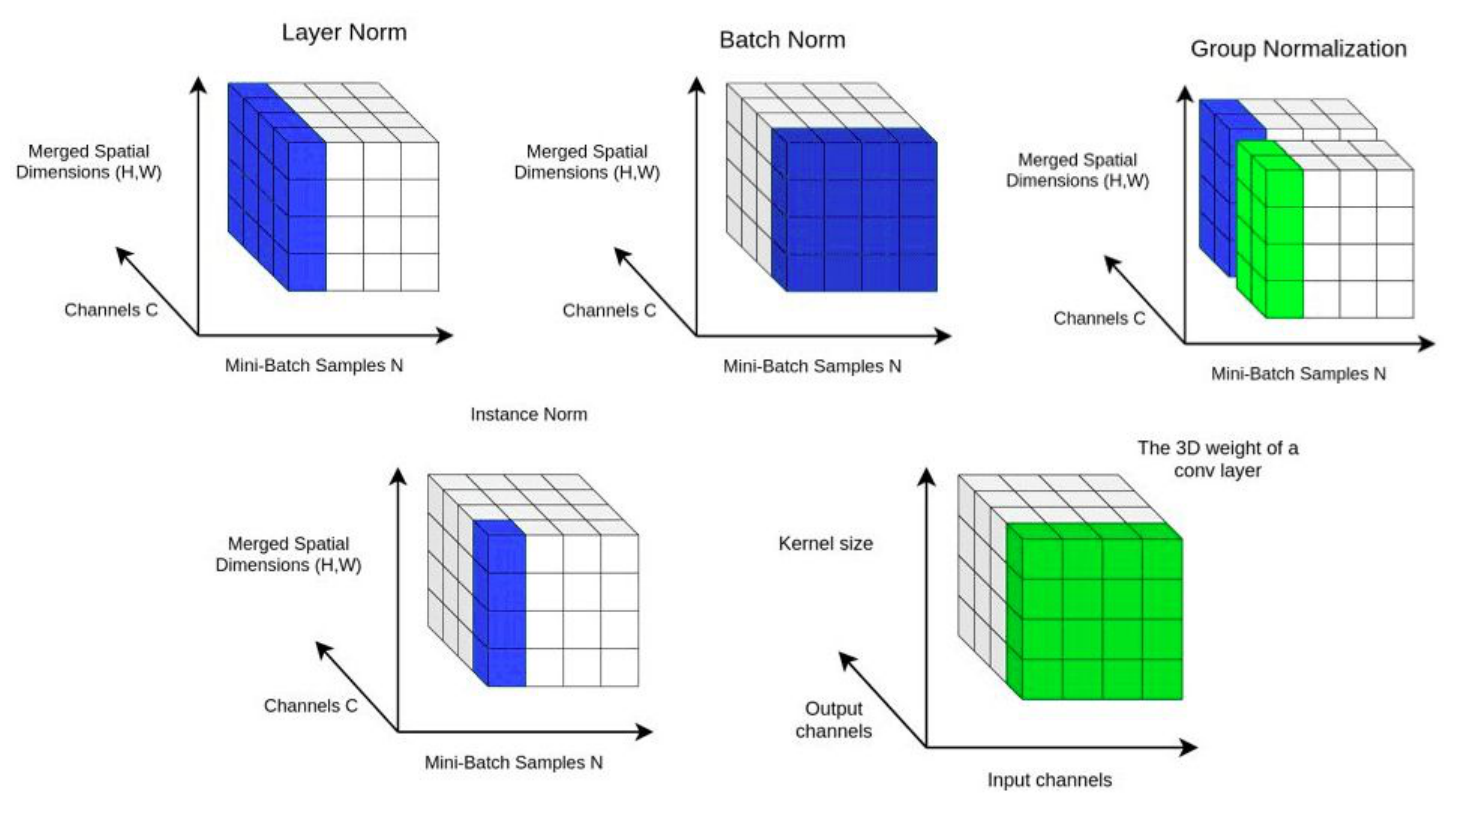
\includegraphics[width=0.8\paperwidth,height=0.8\paperheight,keepaspectratio]{images/introduction-to-transformers/transformer_layer_batch_group_instance_normalization_comparison.png}
\end{frame}

\begin{frame}{Layer Normalization vs RMSNorm}
  \centering
  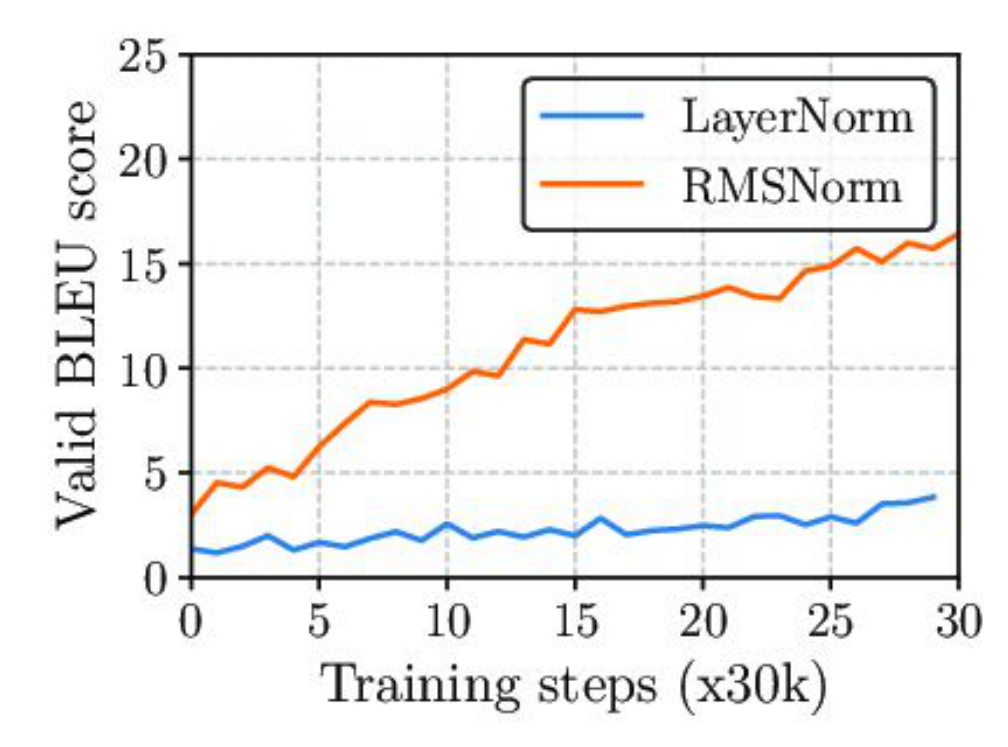
\includegraphics[width=0.8\paperwidth,height=0.8\paperheight,keepaspectratio]{images/introduction-to-transformers/transformer_layer_norm_vs_rms_norm_bleu_curve.png}
\end{frame}

